% Classe do documento e parâmetros gerais.
\documentclass[a4paper,openright,twoside,11pt]{report}

% Packages utilizadas e respetivos parâmetros.
\usepackage[utf8]{inputenc}
\usepackage[english]{babel}
\addto{\captionsenglish}{\renewcommand{\bibname}{References}}
\addto{\captionsenglish}{\renewcommand{\contentsname}{Contents}}
\addto{\captionsenglish}{\renewcommand{\appendixname}{Appendix}}

\usepackage{lipsum} % gerador de texto
\usepackage{graphicx}
\usepackage{url}
\usepackage[Algoritmo]{algorithm}
\usepackage{algorithmicx}
\usepackage{algpseudocode}
\renewcommand{\algorithmicrequire}{\textbf{Dados: }}
\renewcommand{\algorithmicensure}{\textbf{Resultado: }}

% Definições das dimensões das páginas
\setlength{\textheight}{24.00cm}
\setlength{\textwidth}{15.50cm}
\setlength{\topmargin}{0.35cm}
\setlength{\headheight}{0cm}
\setlength{\headsep}{0cm}
\setlength{\oddsidemargin}{0.25cm}
\setlength{\evensidemargin}{0.25cm}

%\renewcommand{\baselinestretch}{1}

% Página inicial (capa)
\title{
   \vspace{-50mm}
   \begin{minipage}[l]{\textwidth}
      \hspace{-20mm}\resizebox{75mm}{!}{
\includegraphics{../../img/figures/logoISELnew2.png}}\\
   \end{minipage}\\[20mm]
   {\bf Remote Lab}
}

% Nome dos autores (um por linha)
\author{
\begin{tabular}{ll}
             & António Alves  \\
             & Ângelo Azevedo \\[50mm]
\end{tabular}}

\date{
\begin{tabular}{ll}
  {Advisor:} & Pedro Matutino \\
\end{tabular}\\[10mm]
% Deixar o indicador respetivo em função da versão do relatório.
Report for Project and Seminar Class\\
Computer Science and Computer Engineering BSc\\[20mm]
June 2025}

\begin{document}
\pagenumbering{roman}
\thispagestyle{empty}
\maketitle

\baselineskip 18pt % line spacing: 12pt for single, 18pt for 1 1/2, and 24pt for double spacing

\newpage
\thispagestyle{empty}
% Fim da contracapa

% Página com identificação completa (número e nome) e assinaturas do(s) estudante(s) e do(s) orientador(es)
\cleardoublepage
\setcounter{page}{1}
\begin{center}
\textsc{\LARGE Lisbon School of Engineering}\\[50mm]

{\large \bf  Remote Lab}\\[20mm]

\begin{tabular}{rl}
  50539  & António Alves\\[10mm]
           & \rule{75mm}{0.5pt}\\[5mm]
  50565  & Ângelo Azevedo\\[10mm]
           & \rule{75mm}{0.5pt}\\
\end{tabular}\\[10mm]

\begin{tabular}{rl}
  Advisor: & Pedro Matutino\\[10mm]
                & \rule{75mm}{0.5pt}\\[5mm]
\end{tabular}\\[10mm]

Report for Project and Seminar Class\\
Computer Science and Computer Engineering BSc\\[20mm]
June 2025\\
\end{center}

% Página de resumo em Português
\cleardoublepage
\chapter*{Abstract}
The design, development, implementation, and finally, the validation of digital systems re-
quire, in addition to simulators, the use of hardware to verify their implementations in real
devices. In the current teaching paradigm, in which face-to-face time is reduced and remote
and autonomous work is increased, it is necessary to create alternatives to the current model.
The Remote Lab project aims to provide a virtual lab with access to remote hardware.
This lab consists of a web application running on an embedded system. The web application,
accessed via a website, aims to provide a dashboard where users can join a laboratory. This
is where users can control the remote hardware. A hierarchy system will be implemented to
provide different roles, each with their own permissions relative to how users can browse the
information provided by the web application.

%{\bf Palavras-chave:} lista de palavras-chave separadas por ;.

%% Página de agradecimentos
%\cleardoublepage
%\chapter*{Agradecimentos}
%Texto dos agradecimentos. É opcional.\\

% Geração do índice de conteúdos
\cleardoublepage
\tableofcontents \cleardoublepage

% Geração do índice de figuras e de tabelas
\listoffigures \cleardoublepage
\listoftables \cleardoublepage

% Reiniciar a numeração de páginas
\setcounter{page}{1}
\pagenumbering{arabic}

% Capitulo 1
%
% Chapter 1
%
\chapter{Introduction} \label{cap:intro}

This is the beginning of the chapter.

Example of indentation of the second paragraph.

%
% Secção 1.1
%
\section{Nome da secção deste capítulo} \label{sec11}

Texto da secção. Na figura~\ref{fig:logotipo} mostra-se o logótipo do ISEL. Em \cite{wiki:bigdata2019} encontra várias referências para o assunto. O artigo \cite{6547630} é o mais popular conforme indicação do IEEE. Logo a seguir aparece \cite{6824752}. A identificação das referências deve ser melhorada.

% Colocar uma figura
\begin{figure}[h]
\begin{center}
%\resizebox{100mm}{!}{\includegraphics{./figures/logoISELnew3.png}}
\end{center}
\caption{Legenda da figura com o logótipo do ISEL.}\label{fig:logotipo}
\end{figure}

Continuação do texto depois do parágrafo que refere a figura.


%
% Secção 1.2
%
\section{A segunda secção deste capítulo} \label{sec12}
Na segunda secção deste capítulo, vamos abordar o enquadramento,
o contexto e as funcionalidades.

%
% Secção 1.2.1
%
\subsection{A primeira sub-secção desta secção} \label{sec121}
As sub-secções são úteis para mostrar determinados conteúdos de forma
organizada. Contudo, o seu uso excessivo também não contribui para a facilidade
de leitura do documento.

%
% Secção 1.2.2
%
\subsection{A segunda sub-secção desta secção} \label{sec122}
Esta é a segunda sub-secção desta secção, a qual termina aqui.


%
% Secção 1.3
%
\section{Organização do documento} \label{sec13}
O restante relatório encontra-se organizado da seguinte forma.

% Capitulo 2
%
% Chapter 3
%
\chapter{Proposed Architecture} \label{cap:proposed-architecture}

This chapter presents the proposed architecture for the Remote Lab platform, detailing its main components, their interactions, and the rationale behind the architectural choices.

%
% Section 3.1
%
\section{System Overview} \label{sec31}
The Remote Lab platform is designed as a modular and scalable system, enabling secure and efficient remote access to laboratory equipment. The architecture follows a layered approach, separating concerns between the user interface, application logic, and hardware integration. This separation facilitates maintainability, extensibility, and the integration of new features or laboratory devices.

%
% Section 3.2
%
\section{Main Components} \label{sec32}
The architecture consists of the following main components:
\begin{itemize}
    \item \textbf{Frontend:} A web-based user interface developed with Next.js, providing users with access to laboratory resources, session scheduling, and experiment monitoring.
    \item \textbf{Backend:} Implemented in Kotlin, the backend exposes RESTful APIs for user management, authentication, authorization, and laboratory session control. It also handles business logic and enforces security policies.
    \item \textbf{Hardware Abstraction Layer:} This layer manages communication with laboratory equipment, abstracting hardware-specific details and providing a unified interface for the backend.
    \item \textbf{Database:} Stores user data, session information, access logs, and configuration settings. The database ensures data consistency and supports auditing requirements.
    \item \textbf{Authentication and Authorization:} Ensures secure access to the platform, supporting multiple user roles (e.g., students, professors, administrators) with different permissions.
\end{itemize}

%
% Section 3.3
%
\section{Component Interactions} \label{sec33}
The components interact as follows:
\begin{itemize}
    \item Users interact with the frontend to authenticate, schedule sessions, and access laboratory resources.
    \item The frontend communicates with the backend via secure API calls.
    \item The backend processes requests, applies business logic, and interacts with the database and hardware abstraction layer as needed.
    \item The hardware abstraction layer translates backend commands into device-specific instructions, enabling remote control of laboratory equipment.
\end{itemize}

%
% Section 3.4
%
\section{Architecture Diagram} \label{sec34}
Figure~\ref{fig:architecture} illustrates the high-level architecture of the Remote Lab platform.

% Insert architecture diagram here
\begin{figure}[h]
\begin{center}
    \resizebox{100mm}{!}{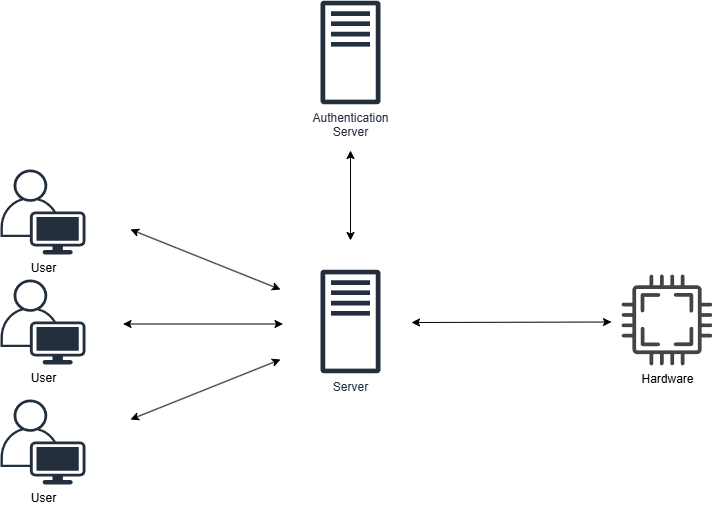
\includegraphics{./../img/SimpleArchitectureRL.drawio.png}}
\end{center}
\caption{High-level architecture of the Remote Lab platform.}\label{fig:architecture}
\end{figure}

%
% Section 3.5
%
\section{Design Rationale} \label{sec35}
The architectural choices were guided by the need for scalability, security, and ease of integration with diverse laboratory equipment. The use of a layered architecture and standardized interfaces ensures that the platform can evolve to meet future requirements and support additional functionalities.
%%
% Capítulo 2
%
\chapter{Enquadramento} \label{cap:enquadramento}

Este capítulo está organizado em duas secções onde se descreve o trabalho relacionado e alguns sistemas semelhantes ao sistema desenvolvido.

\section{Trabalho relacionado}
\lipsum[1-2]

\section{Sistemas semelhantes}
\lipsum[3-5]


% Capitulo 3
%\chapter{Exemplos} \label{cap:exemplos}

A nossa solução é apresentada neste capítulo. A solução consiste em grandes ideias, desenvolvidas e testadas.

Exemplo de indentação do segundo parágrafo.

\section{Nome da primeira secção deste capítulo} \label{sec31}
Texto da secção. Seguem-se exemplos de vários parágrafos.

Esta unidade curricular funciona no semestre de Verão de cada ano letivo. Nos casos de impedimento prolongado justificado (designadamente por doença ou por motivos profissionais no caso dos trabalhadores-estudantes), poderá ser prolongada, havendo lugar à elaboração de outro relatório de progresso
e a nova inscrição se o prolongamento for além do período de época especial desse semestre. A entrega da justificação e a sua apreciação deverão ocorrer antes do final do prazo estabelecido para a entrega final.

O estudante só poderá frequentar Projecto e Seminário se, em conjunto com as restantes unidades curriculares em que se inscreve nesse semestre isso corresponder, no máximo, a 44 créditos ECTS, tendo acumulado, pelo menos, 138 créditos. No caso de estudantes em regime de tempo parcial, o valor máximo
está limitado a 30 créditos no ano letivo. Não são admitidas inscrições como unidade curricular isolada.

Anualmente é divulgada a lista de ideias para projetos e respetivos orientadores. Os estudantes poderão propor outras ideias identificando os orientadores. A escolha da ideia de projeto é feita no período de
interrupção letiva após o semestre de Inverno. As propostas de projeto são registadas no início do período letivo do semestre de Verão, verificado que os estudantes reúnem as condições de frequência.
O projeto deve ser realizado em grupo de dois estudantes (excecionalmente um ou três). Cada elemento do grupo tem tarefas específicas pelas quais é responsável. Esta situação deve ficar clara desde o início do projeto.

A orientação dos projetos é feita por docentes da área departamental onde o curso está ancorado ou por especialistas externos, podendo haver coorientadores, mas sendo obrigatória a coorientação por docente da área departamental no caso de orientação externa. O desenvolvimento do projeto é acompanhado de reuniões periódicas do orientador (ou coorientadores) com o grupo. A informação referente ao projeto é mantida em formato eletrónico em local acessível pelos elementos do grupo, pelos orientadores e pelos docentes de Projecto e Seminário.\\

A avaliação de Projecto e Seminário envolve:
\begin{enumerate}
	\item proposta do projeto;
	\item relatório de progresso;
	\item apresentação individual;
	\item cartaz e versão beta do projeto;
	\item relatório de projeto e discussão pública final.
\end{enumerate}

A avaliação incide sobre o trabalho planeado e desenvolvido pelos estudantes, com constrições de tempo e prazos previamente estabelecidos. Se durante a realização do projeto for considerado que este está em risco, ouvidos os estudantes envolvidos, o orientador e o docente da unidade curricular decidem se o projeto continua. Em caso de desistência do estudante, esta deve ser comunicada ao orientador do projeto e ao regente da unidade curricular.

\section{A segunda secção deste capítulo} \label{sec32}
Na segunda secção deste capítulo, vamos abordar o enquadramento,
o contexto e as funcionalidades.

\subsection{A primeira sub-secção desta secção} \label{sec321}
As sub-secções são úteis para mostrar determinados conteúdos de forma
organizada. Contudo, o seu uso excessivo dificulta a leitura do documento.

\subsection{A segunda sub-secção desta secção} \label{sec322}
Esta é a segunda sub-secção desta secção, a qual termina aqui.

\section{Descrição detalhada da solução} \label{sec33}
A solução proposta assenta nas seguintes ideias. O algoritmo~\ref{alg1}
apresenta as ações de pesquisa de um elemento $E$ sobre um grafo $G$.
\begin{algorithm}
\caption{Algoritmo de pesquisa em grafo.}
\label{alg1}
\algorithmicrequire{Grafo G, Elemento E}\\
\algorithmicensure{Localização de E em G}\\
\begin{enumerate}
\item Para todos os vértices $v$ em $G$
\item Pesquisar e obter a localização de $E$
\begin{enumerate}
	\item Iniciar a lista de pontos, $P$
	\item Ordenar $P$
\end{enumerate}	
\end{enumerate}
\end{algorithm}

\newpage
Nalgumas situações, é necessário apresentar excertos de
código que ilustrem aspetos relevantes da implementação.

\begin{verbatim}
namespace ps;
public static void main() {
		System.out.println(``PS - Projecto e Seminário'');
}
\end{verbatim}

% Capitulo 4
%\chapter{Testes} \label{cap:testes}

Este é o capítulo de testes. 
É possível forçar a inclusão de todas as referências com \cite{*}.

Modo de matemática em texto $x = ma^2$ e em equação (duas formas):
\[
    x = ma^2
\]

\begin{equation}
    x = ma^2
\end{equation}

% Referências
\bibliographystyle{unsrt}
\bibliography{references}
\addcontentsline{toc}{chapter}{References}

% Apêndices (opcional)
\appendix
%%
% Apêndice 1
%
\chapter{Exemplo de apêndice} \label{ap:exemplo}
Este é o primeiro parágrafo do apêndice.


\lipsum[14-16]

\end{document}